\chapter{}
\section{}\begin{enumerate}%Section 4.1

\item  We have a theorem that says that a continuous function on a closed interval has an absolute maximum and minimum.  But remember that to apply a theorem, the hypotheses have to be checked first.  What happens if we eliminate one of those hypotheses?  Consider a discontinuous function on a closed interval.
\begin{enumerate}
	\item Find such a function with a minimum but no maximum.
	\item Find such a function with a maximum but no minimum.
	\item Find such a function with neither a maximum nor minimum.
	\item Find such a function with both a maximum and minimum.  \cite{SBS}
	\item Discuss your observations.
\end{enumerate}

\item  We have a theorem that says that a continuous function on a closed interval has an absolute maximum and minimum.  But remember that to apply a theorem, the hypotheses have to be checked first.  What happens if we eliminate one of those hypotheses?  Consider a continuous function on an open interval.
\begin{enumerate}
	\item  Find such a function with a minimum but no maximum.
	\item Find such a function with a maximum but no minimum.
	\item Find such a function with neither a maximum nor minimum.
	\item Find such a function with both a maximum and minimum.  \cite{SBS}
	\item Discuss your observations. 
\end{enumerate}

\item  Consider this problem: What is the largest possible area for a right triangle whose hypotenuse is 5 cm long?  In this problem, what is the function you are trying to optimize?  What is the constraint(s)?  Explain these 2 equations, how you use them, their relationship to each other, how you know which is which, etc.



\end{enumerate}
\section{}
\begin{enumerate}%Section 4.2

\item  Compare and contrast the Intermediate Value Theorem (IVT) and the Mean Value Theorem (MVT).  

\item  Explain how the Mean Value Theorem can be used to prove that, if $f'\left( x \right) = 0$ for all $x$, then $f$ is a constant function.


\end{enumerate}
\section{}
\begin{enumerate}%Section 4.3

\item  What is the first-derivative test?  How do you use it?  Why does it work?  What does it tell you?  What do you need to be careful about?

\item  Sketch a curve for which $f(x) < 0$, $f'(x)< 0$, and $f'(x)$ is decreasing on $(-\infty, \infty)$.

\item  What is the second-derivative test?  How do you use it?  Why does it work?  What does it tell you?  What do you need to be careful about?



\end{enumerate}
\section{}
\begin{enumerate}%Section 4.4

\item  Find constants a and b that guarantee that the graph of the function defined by $$f(x) = {{ax + 5} \over {3 - bx}}$$ will have a vertical asymptote at $x = 5$ and a horizontal asymptote at 
$y = -3$. \cite{SBS}  In general, discuss how the values of $a$, $b$, $c$ and $d$ determine the horizontal and vertical asymptotes of $$f(x) = {{ax + d} \over {bx + c}}.$$


\item  While studying for an exam, a friend says that a graph is not allowed to touch an asymptote.  What do you think?



\item  Investigate the validity of this statement:  Every rational function has vertical asymptotes.



\end{enumerate}
\section{}
\begin{enumerate}%Section 4.5

\item  You and a friend decide to compare homework and you find the following results.
\begin{center}{Your friend's paper}\end{center}
	$$\begin{array}{rcl}  \displaystyle{\mathop {\lim }\limits_{x \to 3} {{x - 3} \over {x^2  - 3}}}& = &\displaystyle{\mathop {\lim }\limits_{x \to 3} {1 \over {2x}}} \cr  \mbox{}&&\cr  &= &{1 \over 6} \cr \end{array}$$

\begin{center}Your paper\end{center}
$$\begin{array}{rcl}  \displaystyle{\mathop {\lim }\limits_{x \to 3} {{x - 3} \over {x^2  - 3}}} &=& \displaystyle{{0 \over 6}} \cr   \mbox{}&&\cr  &=& 0 \cr\end{array} $$
Who is right?  \cite{FWG}

\item Provide an annotated calculation of $$
\mathop {\lim }\limits_{x \to 1} x^{{1 \mathord{\left/
 {\vphantom {1 {(1 - x)}}} \right.
 \kern-\nulldelimiterspace} {(1 - x)}}} .
$$

\item  The graphs of differentiable functions $f$ and $g$ are shown in Figure \ref{Chapter4Figurec}.  Which of the following is true about $$\mathop {\lim }\limits_{x \to 0} {{f(x)} \over {g(x)}}?$$ \begin{enumerate}\item The limit is less than 0.  \item   The limit is 0.  
\item The limit is 1. \item The limit is greater than 1.  \item The limit does not exist. \end{enumerate}
Explain your solution.  Create another figure similar to Figure \ref{Chapter4Figurec} that would use the same reasoning but would arrive at another answer on the list.  Explain the solution.

%put Chapter4Figc.jpg here
\begin{figure}[ht]
	\centering
		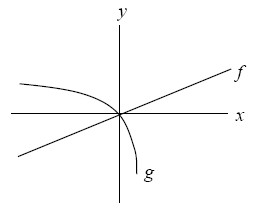
\includegraphics{C:/TeXGraphics/Chapter4Figc.jpg}
	\caption{Two functions}
	\label{Chapter4Figurec}
\end{figure}




\end{enumerate}

